\section{Degradados}

CSS3 permite que se establezca una transición suave o lisa entre dos o más colores. Estos tipos de transiciones o degradados están categorizados en dos tipos: \textbf{lineal} y \textbf{radial}.


\subsection{Degradado lineal}

Para crear un degradado lineal, se utiliza el método \textbf{linear-gradient()}, se deben establecer dos \textbf{escalas de colores}, estas dos escalas de colores renderizarán la transición suave; a estos degradados se le puede establecer un punto de origen y una dirección (o un ángulo). Veamos un ejemplo y su resultado en la \textit{Figura \ref{fig: 42}}:
\begin{lstlisting}
estilos.css
    div {
        width: 300px; 
        height: 100px;
        color: gray;  
        /* Degradado lineal blanco y negro. */
        background: -moz-linear-gradient(black, white);
        font-size: larger;
    }

prueba.html
    <div>
        Hola mundo
    </div>
\end{lstlisting}
\begin{figure}[H]
    \centering
    \caption{Utilizando el degradado lineal simple}
    \label{fig: 42}
    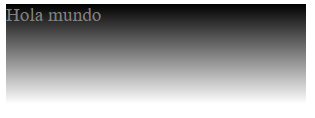
\includegraphics[width=7cm]{ss/linear-gradient-1.png}
\end{figure}


\subsubsection{Prefijos, múltiples escalas y presencia en el degradado}

El ejemplo anterior tiene el \textbf{prefijo del buscador} de Mozilla Firefox, para que este degradado funcione dentro de dicho buscador, pero puede ser agregado, removido o cambiado por otro prefijo en caso de ser requerido. Para el caso de estos apuntes y prácticas, los degradados fueron creados con el buscador \textbf{Microsoft Edge}, el cual no requirió de un prefijo.

En el caso anterior, utilizamos solamente dos escalas de colores con sus respectivas palabras reservadas, pero podemos agregar más de dos, simplemente se agregan separando las escalas por comas, de igual manera, podemos tener, por ejemplo, cinco colores, pero queremos que el cuarto sea el que aparezca más en el degradado, podemos conseguir esto agregando una \textbf{Longitud} (\%, px, pt, cm, em, etc.), como se ve a continuación (\textit{Figura \ref{fig: 43}}):
\begin{lstlisting}
estilos.css
    div {
        width: 500px; 
        height: 300px;
        color: white;
        /* Degradado lineal blanco, negro, rojo y azul al 50% y añade verde. */
        background: linear-gradient(black, white, red, blue 50%, green);
        font-size: larger;
    }

prueba.html
    <div>
        Hola mundo
    </div>
\end{lstlisting}
\begin{figure}[H]
    \centering
    \caption{Utilizando el degradado lineal múltiple}
    \label{fig: 43}
    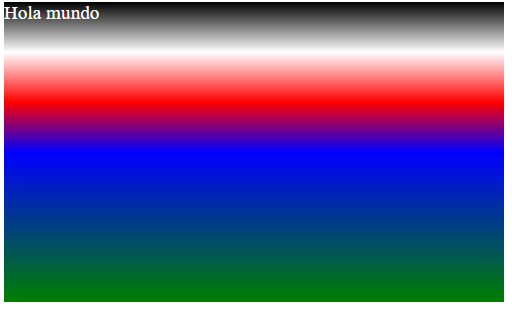
\includegraphics[width=7cm]{ss/linear-gradient-2.png}
\end{figure}

Como vemos, el cuarto color (azul) es el que tiene más presencia, debido a que le asignamos que tuviera una presencia del 50\%.


\subsubsection{Dirección o ángulo del degradado}
\
Podemos lograr que el degradado comience desde distintas \textbf{ubicaciones} del elemento: izquierda, derecha, arriba o abajo, las palabras reservadas \textbf{left}, \textbf{right}, \textbf{top} y \textbf{bottom} respectivamente (también podemos utilizar las esquinas del elemento, por ejemplo, la esquina superior izquierda, que sería \textbf{top left}). 

Considere que, si no utiliza los \textit{prefijos de un buscador}, debe agregar la palabra reservada \textbf{to} previo al valor de dirección predeterminado escogido, si sí va a utilizar un prefijo, no agregue \textbf{to}.
\begin{center}
    \textit{
        // Sin prefijo: \\
        background: linear-gradient(to left, red, blue); \\
        // Con prefijo: \\
        background: -moz-linear-gradient(left, red, blue);
    }
\end{center}

Por otro lado, una alternativa a estas palabras predefinidas son los ángulos, que puede ir desde 0 a 360 grados, si escribimos el valor \textit{0deg}, creará un degradado de izquierda a derecha, mientras que si escribimos el valor \textit{90deg}, creará un degradado de abajo a arriba, experimente con los distintos valores para crear un degradado de su agrado.

Veamos como se ven estas dos formas de dirección en el siguiente ejemplo y su resultado en la \textit{Figura \ref{fig: 44}}:
\begin{lstlisting}
estilos.css
    #dir {
        width: 500px; 
        height: 300px;
        color: white;  
        /* Dirección de degradado con palabras reservadas. */
        background: linear-gradient(to bottom left, red, blue, green);
        font-size: larger;
    }
    
    #ang {
        width: 500px; 
        height: 300px;
        color: white;
        /* Dirección de degradado con ángulos. */
        background: linear-gradient(56deg, pink, purple, orange);
        font-size: larger;
    }

prueba.html
    <div id="dir">
        Con palabras predefinidas
    </div>
    <div id="ang">
        Con ángulos
    </div>
\end{lstlisting}
\begin{figure}[H]
    \centering
    \caption{Utilizando el degradado lineal con dirección}
    \label{fig: 44}
    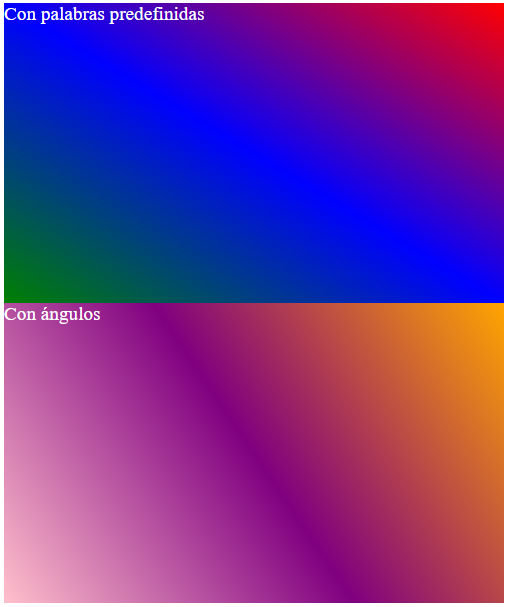
\includegraphics[width=7cm]{ss/linear-gradient-3.png}
\end{figure}


\subsubsection{Repetir el degradado}

Puede repetir un degradado en un mismo elemento con el método \textbf{repeating-linear-gradiant()}, añadiendo una \textbf{Longitud} (\%, px, pt, cm, em, etc.) después de la escala de color. Esta propiedad también acepta las direcciones de degradado. Veamos un ejemplo y su resultado en la \textit{Figura \ref{fig: 45}}:
\begin{lstlisting}
estilos.css
    div {
        width: 500px; 
        height: 300px;
        color: white;
        /* Repite el degradado azul y verde a un 30%. */
        background: repeating-linear-gradient(blue, green 30%);
        font-size: larger;
    }
    
prueba.html
    <div>
        Hola mundo
    </div>
\end{lstlisting}
\begin{figure}[H]
    \centering
    \caption{Repitiendo un degradado lineal}
    \label{fig: 45}
    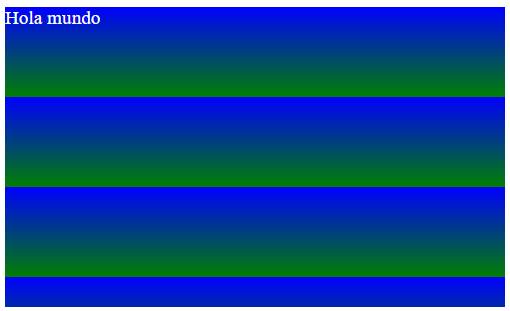
\includegraphics[width=7cm]{ss/linear-gradient-4.png}
\end{figure}

Tomamos el 30\% del tamaño del elemento y metemos ahí al degradado, así con el siguiente 30\% y así sucesivamente.


\subsection{Degradado radial}

La otra manera de definir un degradado a un elemento es por medio del método \textbf{radial-gradient()}, el cual tiene la siguiente sintaxis:
\begin{center}
    \textit{radial-gradient(forma tamaño \textbf{at} posición, escalas de colores);}
\end{center}

Donde:
\begin{itemize}
    \item \textbf{forma}: indica la forma del degradado. Los valores aceptados son \textit{ellipse} (por defecto) y \textit{circle}.
    \item \textbf{tamaño}: indica el tamaño del degradado. Los valores aceptados son \textit{farthest-corner} (por defecto), \textit{closest-side}, \textit{closest-corner} y \textit{farthest-side}.
    \item \textbf{posición}: indica donde comienza el degradado. Se pueden utilizar palabras reservadas (top, bottom, left, right o una combinación de estas) o Unidades de valores, la unidad más común a utilizar es el porcentaje (\%), por ejemplo, 0\%, 0\% hace que el degradado comience en la esquina superior izquierda; 50\%, 50\% hace que comience a la mitad. El valor por defecto es centrado (si es que este parámetro es omitido).
    \item \textbf{escala de colores}: indica los colores del degradado; se pueden poner más de dos, separados por comas, además, se puede repetir los colores como con el estilo de degradado anterior.
\end{itemize}

Mostramos a continuación algunos ejemplos en la \textit{Figura \ref{fig: 46}}:
\begin{lstlisting}
estilos.css
    /* Despliega los contenedores uno al lado del otro. */
    .cont {
        display: inline-block;
    }
    /* Crea contenedores de tamaño fijo, con degradado radial de tres colores y forma de elipse. */
    .rad1 {
        display: inherit;
        width: 300px;
        height: 200px;
        background-image: radial-gradient(red, orange, yellow);
    }
    /* Degradado con repetición de colores y forma circular. */
    .rad2 {
        display: inherit;
        width: 300px;
        height: 200px;
        background-image: radial-gradient(circle, pink 10px, purple 91px);
    }
    /* Degradado de cierto tamaño y posición con forma circular. */
    .rad3 {
        display: inherit;
        width: 300px;
        height: 200px;
        background-image: radial-gradient(circle farthest-side at 30% 70%, blue, green, aqua);
    }

prueba.html
    <div class="cont">
        <div class="rad1"></div>
        <div class="rad2"></div>
        <div class="rad3"></div>
    </div>
\end{lstlisting}
\begin{figure}[H]
    \centering
    \caption{Utilizando el degradado radial}
    \label{fig: 46}
    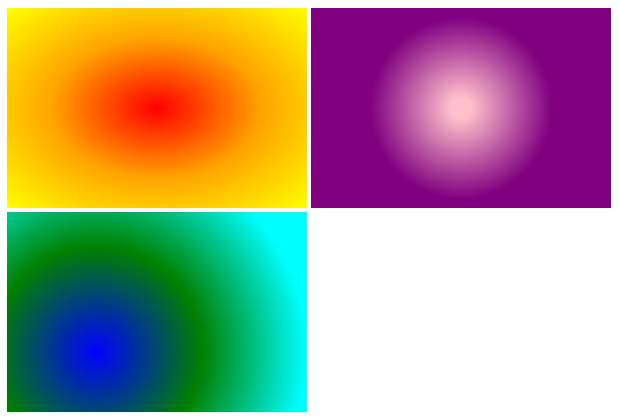
\includegraphics[width=10cm]{ss/radial-gradient.png}
\end{figure}

Como se puede apreciar, se combina la sintaxis de esta función en los tres ejemplos anteriores.



\section{Fondos}


\subsection{background-size}

La propiedad \textbf{background-size} de CSS permite cambiar el tamaño del fondo de un elemento mediante el escalado de la imagen. La mayoría de buscadores ya soportan esta propiedad, por lo que no es necesario agregar un \textit{Prefijo del buscador}. Esta propiedad acepta Unidades de valores o tres palabras reservadas:
\begin{itemize}
    \item \textbf{auto}: por defecto, establece el tamaño de la imagen del fondo tal cual es.
    \item \textbf{contains}: hace que el alto de la imagen del fondo y el alto del elemento HTML sean el mismo. Si el ancho de la imagen de fondo es menor al del elemento, repite la imagen, si no lo es, se ajusta.
    \item \textbf{cover}:  Hace que el ancho de la imagen del fondo y el alto del elemento HTML sean el mismo. Si el alto de la imagen de fondo es es menor al del elemento, se ajusta, si no lo es, se recorta la imagen con respecto al tamaño del elemento.
    \item \textbf{Longitudes} (\%, px, pt, cm, em, etc.).
    \item \textbf{inherit}, \textbf{initial} y \textbf{unset}.
\end{itemize}

La diferencia entre \textit{contains} y \textit{cover} se puede ver a continuación en la \textit{Figura \ref{fig: 47}}:
\begin{lstlisting}
estilos.css
    /* Despliega los contenedores uno al lado del otro. */
    .cont {
        display: inline-block;
    }
    .contains {
        display: inherit;
        /* Tamaño de la clase para ejemplificar la propiedad "background-size". */
        width: 400px;
        height: 250px;
        background-image: url(gato.png);
        background-size: contain;
    }
    .cover {
        display: inherit;
        width: 400px;
        height: 250px;
        background-image: url(gato.png);
        background-size: cover;
    }

prueba.html
    <div class="cont">
        <div class="contains"></div>
        <div class="cover"></div>
    </div>
\end{lstlisting}
\begin{figure}[H]
    \centering
    \caption{Diferencia entre los valores \textit{contains} y \textit{cover}}
    \label{fig: 47}
    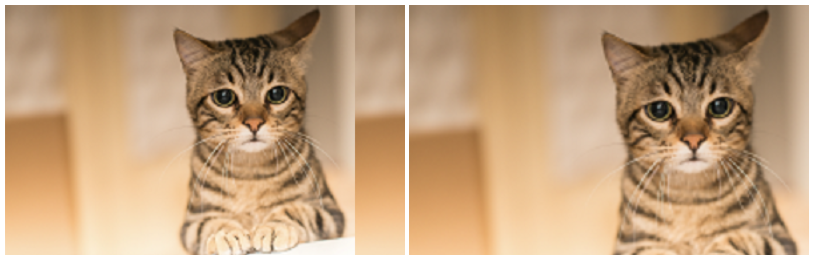
\includegraphics[width=12cm]{ss/background-size.png}
\end{figure}

Como vemos, el ancho del primer elemento es mayor a la imagen de fondo que se le establece, por lo que esta imagen se repite; para el segundo contenedor, el ancho de la imagen y el elemento se ajusta, pero el alto de la imagen de fondo es mayor al alto de su elemento, por lo que la imagen se termina cortando y no mostrándose completamente, esta es la principal diferencia entre ambos valores de la propiedad.


\subsection{background-clip}

La propiedad \textbf{background-clip} de CSS delimita hasta donde se colorea o se aplica una imagen al fondo de un elemento. Los valores aceptados son:
\begin{itemize}
    \item \textbf{border-box}: valor por defecto, colorea o aplica una imagen a un fondo por completo, incluyendo el borde del elemento.
    \item \textbf{padding-box}: colorea o aplica una imagen a un fondo, descartando el padding del elemento.
    \item \textbf{content-box}: colorea o aplica una imagen a un fondo por completo, excluyendo el borde del elemento.
    \item \textbf{initial}, \textbf{unset} y \textbf{inherit}.
\end{itemize}

La diferencia de estos valores se aprecia en la \textit{Figura \ref{fig: 48}}
\begin{lstlisting}
estilos.css
    /* Establece un tipo de borde, padding, color de fondo iguales
    para cada div y la propiedad "background-clip" distinta. */
    #first {
        border: 2px dotted black;
        padding: 20px;
        background: LightBlue;
        background-clip: padding-box;
    }
    #second {
        border: 2px dotted black;
        padding: 20px;
        background: LightBlue;
        background-clip: content-box;
    }
    #third {
        border: 2px dotted black;
        padding: 20px;
        background: LightBlue;
        background-clip: border-box;
    }

prueba.html
    <div id="first">
        <p>background-clip: padding-box</p>
    </div>
    <div id="second">
        <p>background-clip: content-box</p>
    </div>
    <div id="third">
        <p>background-clip: content-box</p>
    </div>
\end{lstlisting}
\begin{figure}[H]
    \centering
    \caption{Diferencia entre los valores \textit{border-box}, \textit{padding-box} y \textit{content-box}}
    \label{fig: 48}
    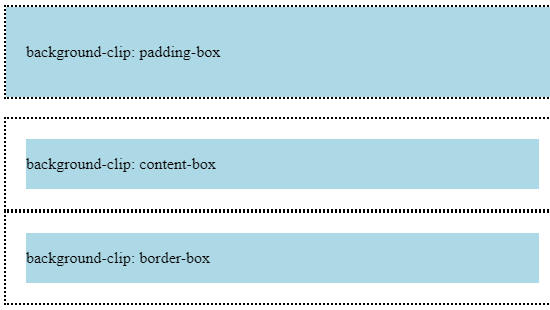
\includegraphics[width=8cm]{ss/background-clip.png}
\end{figure}


\subsection{Bordes transparentes}

Un borde transparente para un elemento se consigue combinando la propiedad \textit{background-clip} y el \textit{RGBA} (\textit{Figura \ref{fig: 49}}):
\begin{lstlisting}
estilos.css
    div {
        /* Borde de 20px de grosor negro y con transparencia de 0.1. */
        border: 20px solid rgba(0, 0, 0, 0.1);
        /* Colorea el borde. */
        background-clip: padding-box; 
        /* Posiciona el div. */
        position:absolute;
        top:50px;
        left:50px;
        width:200px;
        /* Fondo blanco. */
        background-color:white;
    }

prueba.html
    <div>In the screenshot, we set the background-clip to padding-box. The white background ends before the border and the transparency lays over the content</div>

    Some text Some text Some text Some text Some text Some text Some text Some text Some text Some text Some text Some text Some text Some text Some text Some text Some text Some text Some text Some text Some text Some text Some text Some text Some text Some text Some text Some text Some text Some text Some text Some text Some text Some text Some text Some text Some text Some text Some text Some text Some text Some text Some text Some text Some text Some text Some text Some text Some text Some text Some text Some text Some text Some text Some text Some text Some text Some text Some text Some text Some text Some text Some text Some text
\end{lstlisting}
\begin{figure}[H]
    \centering
    \caption{Consiguiendo un borde transparente}
    \label{fig: 49}
    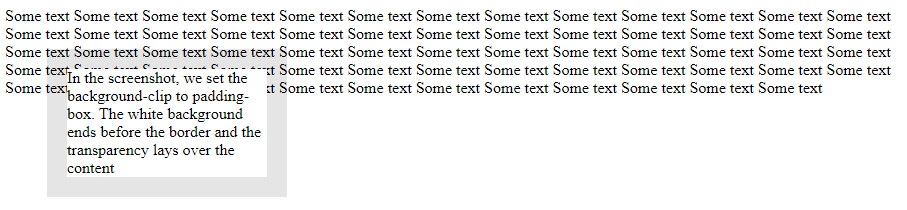
\includegraphics[width=12cm]{ss/borde-transparente.png}
\end{figure}


\subsection{Varias imágenes de fondo}

Podemos poner múltiples fondos a un elemento creando una lista de elementos separados por comas, recordemos que existe el método \textbf{url()}, la cual permite que pongamos un fondo de Internet o del directorio donde estemos trabajando. Las imágenes se van poniendo de \textbf{arriba a abajo}, por lo que la primera irá hasta arriba y la última hasta abajo, como en el siguiente ejemplo (\textit{Figura \ref{fig: 50}}):
\begin{lstlisting}
estilos.css
    div {
        border: 1px solid black;
        width: 400px;
        height: 300px;
        /* Varias imágenes separadas por comas (,). */
        background-image: url("bola.png"), url("gato.png");
        background-position: top, bottom;
        background-repeat: no-repeat;
    }

prueba.html
    <div></div>
\end{lstlisting}
\begin{figure}[H]
    \centering
    \caption{Múltiples fondos}
    \label{fig: 50}
    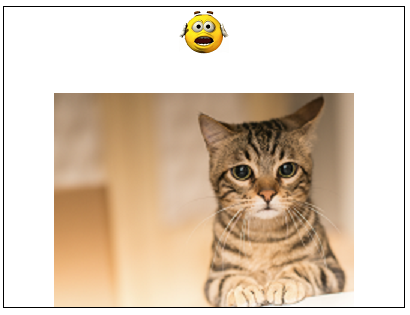
\includegraphics[width=7cm]{ss/multiples-bordes.png}
\end{figure}


\subsubsection{background-position}

Como pudimos ver en el ejemplo anterior, nos saltamos la regla de que los múltiples fondos van de arriba a abajo, los posicionamos distinto mediante una lista separada por comas, esto gracias a la propiedad \textbf{background-position}, esta nos permite establecer la posición de inicio de una imagen de fondo. Los valores aceptados son:
\begin{itemize}
    \item \textbf{left top, left center y left bottom}: comenzando desde la izquierda a arriba, en medio o abajo respectivamente.
    \item \textbf{right top, right center y right bottom}: comenzando desde la derecha a arriba, en medio o abajo respectivamente
    \item \textbf{center top, center center y center bottom}: comenzando del centro a arriba, en medio o abajo respectivamente.
    \item \textbf{Longitudes} (\%, px, pt, cm, em, etc.).
    \item \textbf{initial}, \textbf{unset} y \textbf{inherit}.
\end{itemize}

Los valores con palabra reservada se pueden mezclar, es por eso que los pusimos directamente como \textit{left top}, \textit{right center} o \textit{center bottom}, pero también puede utilizarlos como palabra sola (\textit{top}, \textit{left}, \textit{right} y \textbf{bottom}).

También puede utilizar la propiedad recortada \textit{background} para establecer la imagen, su posición y si se repite o  no:
\begin{center}
    \textit{background: url([imagen]) [posición] [repetir]}
\end{center}


\subsection{opacity}

La propiedad \textbf{opacity} permite volver transparente una imagen de manera sencilla, ya que su valor tope es 1 (opaco) y su valor mínimo es 0 (completamente transparente), por lo que debe establecer un valor decimal entre ambos topes, como se ve en la \textit{Figura \ref{fig: 51}}:
\begin{lstlisting}
estilos.css
    /* Imagen con opacidad de 0.5. */
    #img1 {
        width: 400px;
        height: 400px;
        background-image: url("gato.png");
        background-repeat: no-repeat;
        opacity: 0.5;
    }
    #img2 {
        /* Imagen con opacidad de 0.2. */
        width: 400px;
        height: 400px;
        background-image: url("gato.png");
        background-repeat: no-repeat;
        opacity: 0.2;
    }

prueba.html
    <div id="img1"></div>
    <div id="img2"></div>
\end{lstlisting}
\begin{figure}[H]
    \centering
    \caption{Transparencia de imágenes}
    \label{fig: 51}
    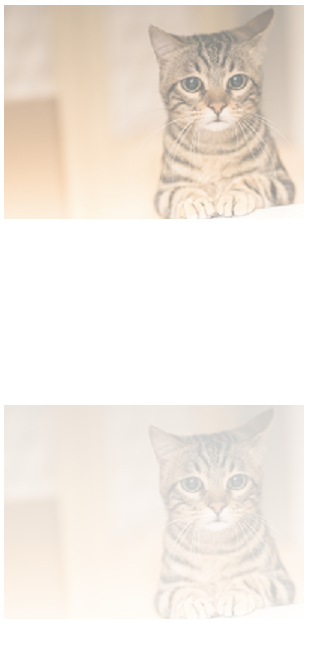
\includegraphics[width=7cm]{ss/opacity.png}
\end{figure}
